% Options for packages loaded elsewhere
\PassOptionsToPackage{unicode}{hyperref}
\PassOptionsToPackage{hyphens}{url}
%
\documentclass[
]{article}
\usepackage{amsmath,amssymb}
\usepackage{lmodern}
\usepackage{iftex}
\ifPDFTeX
  \usepackage[T1]{fontenc}
  \usepackage[utf8]{inputenc}
  \usepackage{textcomp} % provide euro and other symbols
\else % if luatex or xetex
  \usepackage{unicode-math}
  \defaultfontfeatures{Scale=MatchLowercase}
  \defaultfontfeatures[\rmfamily]{Ligatures=TeX,Scale=1}
\fi
% Use upquote if available, for straight quotes in verbatim environments
\IfFileExists{upquote.sty}{\usepackage{upquote}}{}
\IfFileExists{microtype.sty}{% use microtype if available
  \usepackage[]{microtype}
  \UseMicrotypeSet[protrusion]{basicmath} % disable protrusion for tt fonts
}{}
\makeatletter
\@ifundefined{KOMAClassName}{% if non-KOMA class
  \IfFileExists{parskip.sty}{%
    \usepackage{parskip}
  }{% else
    \setlength{\parindent}{0pt}
    \setlength{\parskip}{6pt plus 2pt minus 1pt}}
}{% if KOMA class
  \KOMAoptions{parskip=half}}
\makeatother
\usepackage{xcolor}
\usepackage[margin=1in]{geometry}
\usepackage{color}
\usepackage{fancyvrb}
\newcommand{\VerbBar}{|}
\newcommand{\VERB}{\Verb[commandchars=\\\{\}]}
\DefineVerbatimEnvironment{Highlighting}{Verbatim}{commandchars=\\\{\}}
% Add ',fontsize=\small' for more characters per line
\usepackage{framed}
\definecolor{shadecolor}{RGB}{248,248,248}
\newenvironment{Shaded}{\begin{snugshade}}{\end{snugshade}}
\newcommand{\AlertTok}[1]{\textcolor[rgb]{0.94,0.16,0.16}{#1}}
\newcommand{\AnnotationTok}[1]{\textcolor[rgb]{0.56,0.35,0.01}{\textbf{\textit{#1}}}}
\newcommand{\AttributeTok}[1]{\textcolor[rgb]{0.77,0.63,0.00}{#1}}
\newcommand{\BaseNTok}[1]{\textcolor[rgb]{0.00,0.00,0.81}{#1}}
\newcommand{\BuiltInTok}[1]{#1}
\newcommand{\CharTok}[1]{\textcolor[rgb]{0.31,0.60,0.02}{#1}}
\newcommand{\CommentTok}[1]{\textcolor[rgb]{0.56,0.35,0.01}{\textit{#1}}}
\newcommand{\CommentVarTok}[1]{\textcolor[rgb]{0.56,0.35,0.01}{\textbf{\textit{#1}}}}
\newcommand{\ConstantTok}[1]{\textcolor[rgb]{0.00,0.00,0.00}{#1}}
\newcommand{\ControlFlowTok}[1]{\textcolor[rgb]{0.13,0.29,0.53}{\textbf{#1}}}
\newcommand{\DataTypeTok}[1]{\textcolor[rgb]{0.13,0.29,0.53}{#1}}
\newcommand{\DecValTok}[1]{\textcolor[rgb]{0.00,0.00,0.81}{#1}}
\newcommand{\DocumentationTok}[1]{\textcolor[rgb]{0.56,0.35,0.01}{\textbf{\textit{#1}}}}
\newcommand{\ErrorTok}[1]{\textcolor[rgb]{0.64,0.00,0.00}{\textbf{#1}}}
\newcommand{\ExtensionTok}[1]{#1}
\newcommand{\FloatTok}[1]{\textcolor[rgb]{0.00,0.00,0.81}{#1}}
\newcommand{\FunctionTok}[1]{\textcolor[rgb]{0.00,0.00,0.00}{#1}}
\newcommand{\ImportTok}[1]{#1}
\newcommand{\InformationTok}[1]{\textcolor[rgb]{0.56,0.35,0.01}{\textbf{\textit{#1}}}}
\newcommand{\KeywordTok}[1]{\textcolor[rgb]{0.13,0.29,0.53}{\textbf{#1}}}
\newcommand{\NormalTok}[1]{#1}
\newcommand{\OperatorTok}[1]{\textcolor[rgb]{0.81,0.36,0.00}{\textbf{#1}}}
\newcommand{\OtherTok}[1]{\textcolor[rgb]{0.56,0.35,0.01}{#1}}
\newcommand{\PreprocessorTok}[1]{\textcolor[rgb]{0.56,0.35,0.01}{\textit{#1}}}
\newcommand{\RegionMarkerTok}[1]{#1}
\newcommand{\SpecialCharTok}[1]{\textcolor[rgb]{0.00,0.00,0.00}{#1}}
\newcommand{\SpecialStringTok}[1]{\textcolor[rgb]{0.31,0.60,0.02}{#1}}
\newcommand{\StringTok}[1]{\textcolor[rgb]{0.31,0.60,0.02}{#1}}
\newcommand{\VariableTok}[1]{\textcolor[rgb]{0.00,0.00,0.00}{#1}}
\newcommand{\VerbatimStringTok}[1]{\textcolor[rgb]{0.31,0.60,0.02}{#1}}
\newcommand{\WarningTok}[1]{\textcolor[rgb]{0.56,0.35,0.01}{\textbf{\textit{#1}}}}
\usepackage{graphicx}
\makeatletter
\def\maxwidth{\ifdim\Gin@nat@width>\linewidth\linewidth\else\Gin@nat@width\fi}
\def\maxheight{\ifdim\Gin@nat@height>\textheight\textheight\else\Gin@nat@height\fi}
\makeatother
% Scale images if necessary, so that they will not overflow the page
% margins by default, and it is still possible to overwrite the defaults
% using explicit options in \includegraphics[width, height, ...]{}
\setkeys{Gin}{width=\maxwidth,height=\maxheight,keepaspectratio}
% Set default figure placement to htbp
\makeatletter
\def\fps@figure{htbp}
\makeatother
\setlength{\emergencystretch}{3em} % prevent overfull lines
\providecommand{\tightlist}{%
  \setlength{\itemsep}{0pt}\setlength{\parskip}{0pt}}
\setcounter{secnumdepth}{-\maxdimen} % remove section numbering
\ifLuaTeX
  \usepackage{selnolig}  % disable illegal ligatures
\fi
\IfFileExists{bookmark.sty}{\usepackage{bookmark}}{\usepackage{hyperref}}
\IfFileExists{xurl.sty}{\usepackage{xurl}}{} % add URL line breaks if available
\urlstyle{same} % disable monospaced font for URLs
\hypersetup{
  pdftitle={HW3},
  pdfauthor={Alexandra Gibbons},
  hidelinks,
  pdfcreator={LaTeX via pandoc}}

\title{HW3}
\author{Alexandra Gibbons}
\date{2022-09-16}

\begin{document}
\maketitle

\hypertarget{dv-3}{%
\section{DV 3}\label{dv-3}}

\hypertarget{question-1}{%
\subsection{Question 1}\label{question-1}}

\begin{Shaded}
\begin{Highlighting}[]
\FunctionTok{library}\NormalTok{(tidyverse)}
\end{Highlighting}
\end{Shaded}

\begin{verbatim}
## -- Attaching packages --------------------------------------- tidyverse 1.3.2 --
## v ggplot2 3.3.6     v purrr   0.3.4
## v tibble  3.1.8     v dplyr   1.0.9
## v tidyr   1.2.0     v stringr 1.4.1
## v readr   2.1.2     v forcats 0.5.2
## -- Conflicts ------------------------------------------ tidyverse_conflicts() --
## x dplyr::filter() masks stats::filter()
## x dplyr::lag()    masks stats::lag()
\end{verbatim}

\begin{Shaded}
\begin{Highlighting}[]
\CommentTok{\# Read in the data }
\NormalTok{exercise\_data }\OtherTok{\textless{}{-}} \FunctionTok{read\_csv}\NormalTok{(}\StringTok{"Data/visualize\_data.csv"}\NormalTok{)}
\end{Highlighting}
\end{Shaded}

\begin{verbatim}
## New names:
## Rows: 142 Columns: 4
## -- Column specification
## -------------------------------------------------------- Delimiter: "," dbl
## (4): ...1, ...2, Exercise, BMI
## i Use `spec()` to retrieve the full column specification for this data. i
## Specify the column types or set `show_col_types = FALSE` to quiet this message.
## * `` -> `...1`
## * `...1` -> `...2`
\end{verbatim}

\begin{Shaded}
\begin{Highlighting}[]
\FunctionTok{glimpse}\NormalTok{(exercise\_data)}
\end{Highlighting}
\end{Shaded}

\begin{verbatim}
## Rows: 142
## Columns: 4
## $ ...1     <dbl> 1, 2, 3, 4, 5, 6, 7, 8, 9, 10, 11, 12, 13, 14, 15, 16, 17, 18~
## $ ...2     <dbl> 1, 2, 3, 4, 5, 6, 7, 8, 9, 10, 11, 12, 13, 14, 15, 16, 17, 18~
## $ Exercise <dbl> 55.3846, 51.5385, 46.1538, 42.8205, 40.7692, 38.7179, 35.6410~
## $ BMI      <dbl> 1.8320590, 1.7892194, 1.7321050, 1.6178724, 1.5036362, 1.3751~
\end{verbatim}

I expect that people who record more exercise will have lower BMIs.

\begin{Shaded}
\begin{Highlighting}[]
\FunctionTok{cor}\NormalTok{(exercise\_data}\SpecialCharTok{$}\NormalTok{Exercise, exercise\_data}\SpecialCharTok{$}\NormalTok{BMI)}
\end{Highlighting}
\end{Shaded}

\begin{verbatim}
## [1] -0.06447185
\end{verbatim}

The correlation coefficient is negative, which indicates that an
increase in recorded exercise time is associated with a decrease in BMI.

\begin{Shaded}
\begin{Highlighting}[]
\NormalTok{exercise\_data }\SpecialCharTok{\%\textgreater{}\%} 
  \FunctionTok{ggplot}\NormalTok{(}\FunctionTok{aes}\NormalTok{(}\AttributeTok{x =}\NormalTok{ Exercise, }
              \AttributeTok{y =}\NormalTok{ BMI)) }\SpecialCharTok{+}
  \FunctionTok{geom\_point}\NormalTok{()}
\end{Highlighting}
\end{Shaded}

\includegraphics{HW3_files/figure-latex/unnamed-chunk-3-1.pdf} \#\#
Question 2

\begin{Shaded}
\begin{Highlighting}[]
\FunctionTok{library}\NormalTok{(causact)}
\FunctionTok{glimpse}\NormalTok{(corruptDF)}
\end{Highlighting}
\end{Shaded}

\begin{verbatim}
## Rows: 174
## Columns: 7
## $ country     <chr> "Afghanistan", "Albania", "Algeria", "Angola", "Argentina"~
## $ region      <chr> "Asia Pacific", "East EU Cemt Asia", "MENA", "SSA", "Ameri~
## $ countryCode <chr> "AFG", "ALB", "DZA", "AGO", "ARG", "ARM", "AUS", "AUT", "A~
## $ regionCode  <chr> "AP", "ECA", "MENA", "SSA", "AME", "ECA", "AP", "WE/EU", "~
## $ population  <int> 35530081, 2873457, 41318142, 29784193, 44271041, 2930450, ~
## $ CPI2017     <int> 15, 38, 33, 19, 39, 35, 77, 75, 31, 65, 36, 28, 68, 44, 75~
## $ HDI2017     <dbl> 0.498, 0.785, 0.754, 0.581, 0.825, 0.755, 0.939, 0.908, 0.~
\end{verbatim}

\begin{Shaded}
\begin{Highlighting}[]
\NormalTok{?corruptDF}
\end{Highlighting}
\end{Shaded}

CPI2017 is a country's (or territory's) score on the Corruption
Perceptions Index in 2017, which measures the perception of the level of
corruption in the public sector. Scores range from 0 to 100, with 0
meaning that a given country is percieved as being very corrupt, and a
score of 100 meaning that the country is not percieved as corrupt in the
public sector.

HDI2017 is a country's or territory's Human Development Index score from
2017, which represents human development based on life expectancy,
education levels, and income.

\hypertarget{question-3}{%
\subsection{Question 3}\label{question-3}}

\begin{Shaded}
\begin{Highlighting}[]
\NormalTok{corruptDF }\SpecialCharTok{\%\textgreater{}\%} 
  \FunctionTok{ggplot}\NormalTok{(}\FunctionTok{aes}\NormalTok{(}\AttributeTok{x=}\NormalTok{HDI2017,}
             \AttributeTok{y=}\NormalTok{CPI2017)) }\SpecialCharTok{+}
  \FunctionTok{geom\_point}\NormalTok{()}
\end{Highlighting}
\end{Shaded}

\includegraphics{HW3_files/figure-latex/unnamed-chunk-5-1.pdf}

There seems to be a positive association between HDI and CPI scores in
2017. This relationship doesn't look perfectly linear and may be best
represented with a quadratic function.

\hypertarget{question-4}{%
\subsection{Question 4}\label{question-4}}

\begin{Shaded}
\begin{Highlighting}[]
\NormalTok{corruptDF }\SpecialCharTok{\%\textgreater{}\%} 
  \FunctionTok{ggplot}\NormalTok{(}\FunctionTok{aes}\NormalTok{(}\AttributeTok{x=}\NormalTok{HDI2017,}
             \AttributeTok{y=}\NormalTok{CPI2017)) }\SpecialCharTok{+}
  \FunctionTok{geom\_point}\NormalTok{() }\SpecialCharTok{+}
  \FunctionTok{geom\_smooth}\NormalTok{(}\AttributeTok{method=}\StringTok{"gam"}\NormalTok{)}
\end{Highlighting}
\end{Shaded}

\begin{verbatim}
## `geom_smooth()` using formula 'y ~ s(x, bs = "cs")'
\end{verbatim}

\includegraphics{HW3_files/figure-latex/unnamed-chunk-6-1.pdf}

\begin{Shaded}
\begin{Highlighting}[]
\NormalTok{corruptDF }\SpecialCharTok{\%\textgreater{}\%} 
  \FunctionTok{ggplot}\NormalTok{(}\FunctionTok{aes}\NormalTok{(}\AttributeTok{x=}\NormalTok{HDI2017,}
             \AttributeTok{y=}\NormalTok{CPI2017)) }\SpecialCharTok{+}
  \FunctionTok{geom\_point}\NormalTok{() }\SpecialCharTok{+}
  \FunctionTok{geom\_smooth}\NormalTok{(}\AttributeTok{method=}\StringTok{"lm"}\NormalTok{)}
\end{Highlighting}
\end{Shaded}

\begin{verbatim}
## `geom_smooth()` using formula 'y ~ x'
\end{verbatim}

\includegraphics{HW3_files/figure-latex/unnamed-chunk-6-2.pdf}

The \texttt{gam} method fits a generalized additive model, which is more
flexible and fits this data much better than the \texttt{lm} method,
which fits a simple linear model and thus renders a straight line.

\hypertarget{question-5}{%
\subsection{Question 5}\label{question-5}}

\begin{Shaded}
\begin{Highlighting}[]
\NormalTok{corruptDF }\SpecialCharTok{\%\textgreater{}\%} 
  \FunctionTok{ggplot}\NormalTok{(}\FunctionTok{aes}\NormalTok{(}\AttributeTok{x=}\NormalTok{HDI2017,}
             \AttributeTok{y=}\NormalTok{CPI2017,}
             \AttributeTok{color=}\NormalTok{region,}
             \AttributeTok{fill=}\NormalTok{region)) }\SpecialCharTok{+}
  \FunctionTok{geom\_point}\NormalTok{() }\SpecialCharTok{+}
  \FunctionTok{geom\_smooth}\NormalTok{(}\AttributeTok{method=}\StringTok{"gam"}\NormalTok{)}
\end{Highlighting}
\end{Shaded}

\begin{verbatim}
## `geom_smooth()` using formula 'y ~ s(x, bs = "cs")'
\end{verbatim}

\includegraphics{HW3_files/figure-latex/unnamed-chunk-7-1.pdf}

Haha, this is way too cluttered. Let's try again\ldots{}

\begin{Shaded}
\begin{Highlighting}[]
\NormalTok{corruptDF }\SpecialCharTok{\%\textgreater{}\%} 
  \FunctionTok{ggplot}\NormalTok{(}\FunctionTok{aes}\NormalTok{(}\AttributeTok{x=}\NormalTok{HDI2017,}
             \AttributeTok{y=}\NormalTok{CPI2017)) }\SpecialCharTok{+}
  \FunctionTok{geom\_point}\NormalTok{() }\SpecialCharTok{+}
  \FunctionTok{geom\_smooth}\NormalTok{(}\AttributeTok{method=}\StringTok{"gam"}\NormalTok{) }\SpecialCharTok{+}
  \FunctionTok{facet\_wrap}\NormalTok{(}\SpecialCharTok{\textasciitilde{}}\NormalTok{region)}
\end{Highlighting}
\end{Shaded}

\begin{verbatim}
## `geom_smooth()` using formula 'y ~ s(x, bs = "cs")'
\end{verbatim}

\includegraphics{HW3_files/figure-latex/unnamed-chunk-8-1.pdf}

This is much more digestible.

\hypertarget{question-6}{%
\subsection{Question 6}\label{question-6}}

\begin{Shaded}
\begin{Highlighting}[]
\NormalTok{corruptDF }\SpecialCharTok{\%\textgreater{}\%} 
  \FunctionTok{ggplot}\NormalTok{(}\FunctionTok{aes}\NormalTok{(}\AttributeTok{x=}\NormalTok{HDI2017,}
             \AttributeTok{y=}\NormalTok{CPI2017)) }\SpecialCharTok{+}
  \FunctionTok{geom\_point}\NormalTok{() }\SpecialCharTok{+}
  \FunctionTok{geom\_smooth}\NormalTok{(}\AttributeTok{method=}\StringTok{"gam"}\NormalTok{) }\SpecialCharTok{+}
  \FunctionTok{scale\_x\_reverse}\NormalTok{()}
\end{Highlighting}
\end{Shaded}

\begin{verbatim}
## `geom_smooth()` using formula 'y ~ s(x, bs = "cs")'
\end{verbatim}

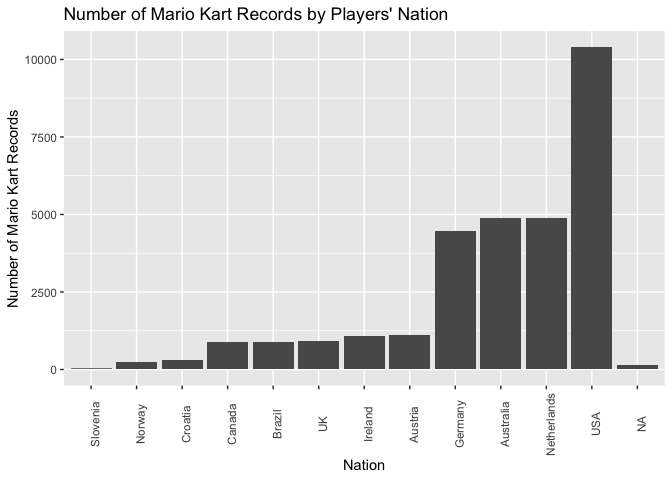
\includegraphics{HW3_files/figure-latex/unnamed-chunk-9-1.pdf}

Done, though I don't particularly like it.

\hypertarget{question-7}{%
\subsection{Question 7}\label{question-7}}

\begin{Shaded}
\begin{Highlighting}[]
\NormalTok{final\_plot }\OtherTok{\textless{}{-}}\NormalTok{ corruptDF }\SpecialCharTok{\%\textgreater{}\%} 
  \FunctionTok{ggplot}\NormalTok{(}\FunctionTok{aes}\NormalTok{(}\AttributeTok{x=}\NormalTok{HDI2017,}
             \AttributeTok{y=}\NormalTok{CPI2017)) }\SpecialCharTok{+}
  \FunctionTok{geom\_point}\NormalTok{() }\SpecialCharTok{+}
  \FunctionTok{geom\_smooth}\NormalTok{(}\AttributeTok{method=}\StringTok{"gam"}\NormalTok{) }\SpecialCharTok{+}
  \FunctionTok{labs}\NormalTok{(}\AttributeTok{x=}\StringTok{"Human Development Index Score"}\NormalTok{,}
       \AttributeTok{y=}\StringTok{"Corruption Perceptions Index Score"}\NormalTok{,}
       \AttributeTok{title=}\StringTok{"Human Development and Corruption Perception in 2017"}\NormalTok{,}
       \AttributeTok{subtitle=}\StringTok{"Data points are countries"}\NormalTok{,}
       \AttributeTok{caption=}\StringTok{"Source: causact package in R"}\NormalTok{)}
\end{Highlighting}
\end{Shaded}

\hypertarget{question-8}{%
\subsection{Question 8}\label{question-8}}

\begin{Shaded}
\begin{Highlighting}[]
\CommentTok{\#setwd("/Users/ajg109//Documents/Github/sociol\_722/HW3")}
\CommentTok{\#ggsave("hw3\_plot.pdf", plot=final\_plot)}
\end{Highlighting}
\end{Shaded}

I commented this out because it was preventing knitting but I promise it
worked and I have since used ggsave to successfully save a graph I made
for work!

\hypertarget{dv-4}{%
\section{DV 4}\label{dv-4}}

\hypertarget{question-1-1}{%
\subsection{Question 1}\label{question-1-1}}

\begin{Shaded}
\begin{Highlighting}[]
\FunctionTok{library}\NormalTok{(tidyverse)}

\CommentTok{\# Read in the data }
\NormalTok{tv\_ratings }\OtherTok{\textless{}{-}} \FunctionTok{read\_csv}\NormalTok{(}\StringTok{"Data/tv\_ratings.csv"}\NormalTok{)}
\end{Highlighting}
\end{Shaded}

\begin{verbatim}
## Rows: 2266 Columns: 7
## -- Column specification --------------------------------------------------------
## Delimiter: ","
## chr  (3): titleId, title, genres
## dbl  (3): seasonNumber, av_rating, share
## date (1): date
## 
## i Use `spec()` to retrieve the full column specification for this data.
## i Specify the column types or set `show_col_types = FALSE` to quiet this message.
\end{verbatim}

\begin{Shaded}
\begin{Highlighting}[]
\CommentTok{\# Glimpse the data }
\FunctionTok{glimpse}\NormalTok{(tv\_ratings)}
\end{Highlighting}
\end{Shaded}

\begin{verbatim}
## Rows: 2,266
## Columns: 7
## $ titleId      <chr> "tt2879552", "tt3148266", "tt3148266", "tt3148266", "tt31~
## $ seasonNumber <dbl> 1, 1, 2, 3, 4, 1, 2, 1, 2, 3, 4, 5, 6, 7, 8, 1, 1, 1, 1, ~
## $ title        <chr> "11.22.63", "12 Monkeys", "12 Monkeys", "12 Monkeys", "12~
## $ date         <date> 2016-03-10, 2015-02-27, 2016-05-30, 2017-05-19, 2018-06-~
## $ av_rating    <dbl> 8.4890, 8.3407, 8.8196, 9.0369, 9.1363, 8.4370, 7.5089, 8~
## $ share        <dbl> 0.51, 0.46, 0.25, 0.19, 0.38, 2.38, 2.19, 6.67, 7.13, 5.8~
## $ genres       <chr> "Drama,Mystery,Sci-Fi", "Adventure,Drama,Mystery", "Adven~
\end{verbatim}

\begin{Shaded}
\begin{Highlighting}[]
\NormalTok{tv\_long }\OtherTok{\textless{}{-}}\NormalTok{ tv\_ratings }\SpecialCharTok{\%\textgreater{}\%} 
  \FunctionTok{group\_by}\NormalTok{(title) }\SpecialCharTok{\%\textgreater{}\%} 
  \FunctionTok{summarise}\NormalTok{(}\AttributeTok{num\_seasons =} \FunctionTok{n}\NormalTok{()) }\SpecialCharTok{\%\textgreater{}\%} 
  \FunctionTok{ungroup}\NormalTok{() }\SpecialCharTok{\%\textgreater{}\%} 
  \FunctionTok{left\_join}\NormalTok{(tv\_ratings, }\AttributeTok{by =} \StringTok{"title"}\NormalTok{) }

\NormalTok{tv\_long }\OtherTok{\textless{}{-}}\NormalTok{ tv\_long }\SpecialCharTok{\%\textgreater{}\%} 
  \FunctionTok{filter}\NormalTok{(num\_seasons }\SpecialCharTok{\textgreater{}=} \DecValTok{5}\NormalTok{)}
\end{Highlighting}
\end{Shaded}

\begin{Shaded}
\begin{Highlighting}[]
\NormalTok{tv\_long }\SpecialCharTok{\%\textgreater{}\%} 
  \FunctionTok{ggplot}\NormalTok{(}\FunctionTok{aes}\NormalTok{(}\AttributeTok{x=}\NormalTok{seasonNumber,}
             \AttributeTok{y=}\NormalTok{av\_rating,}
             \AttributeTok{group=}\NormalTok{title)) }\SpecialCharTok{+}
  \FunctionTok{geom\_line}\NormalTok{() }\SpecialCharTok{+} 
  \FunctionTok{labs}\NormalTok{(}\AttributeTok{x=}\StringTok{"Season Number"}\NormalTok{, }\AttributeTok{y=}\StringTok{"Average Rating"}\NormalTok{) }\SpecialCharTok{+}
  \FunctionTok{theme\_minimal}\NormalTok{()}
\end{Highlighting}
\end{Shaded}

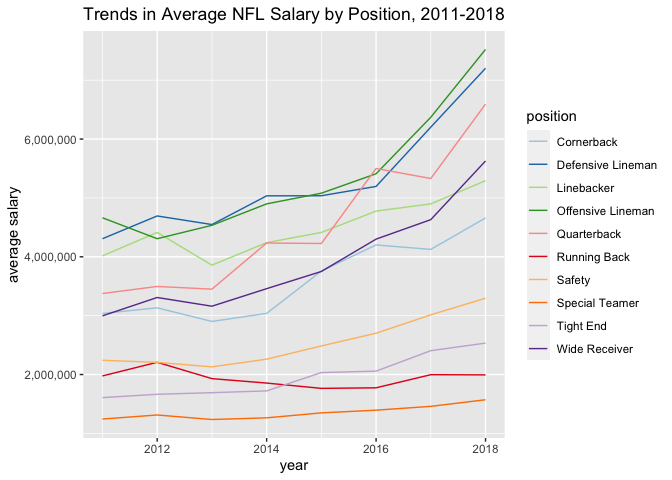
\includegraphics{HW3_files/figure-latex/unnamed-chunk-14-1.pdf}

This graph is extremely messy and it is difficult to draw any
conclusions.

\hypertarget{question-2}{%
\subsection{Question 2}\label{question-2}}

\begin{Shaded}
\begin{Highlighting}[]
\NormalTok{tv\_long }\SpecialCharTok{\%\textgreater{}\%} 
  \FunctionTok{ggplot}\NormalTok{(}\FunctionTok{aes}\NormalTok{(}\AttributeTok{x=}\NormalTok{seasonNumber,}
             \AttributeTok{y=}\NormalTok{av\_rating, }
             \AttributeTok{group=}\NormalTok{title)) }\SpecialCharTok{+}
  \FunctionTok{geom\_line}\NormalTok{() }\SpecialCharTok{+}
  \FunctionTok{facet\_wrap}\NormalTok{(}\SpecialCharTok{\textasciitilde{}}\NormalTok{genres) }\SpecialCharTok{+} 
  \FunctionTok{labs}\NormalTok{(}\AttributeTok{x=}\StringTok{"Season Number"}\NormalTok{, }\AttributeTok{y=}\StringTok{"Average Rating"}\NormalTok{) }\SpecialCharTok{+}
  \FunctionTok{theme\_minimal}\NormalTok{()}
\end{Highlighting}
\end{Shaded}

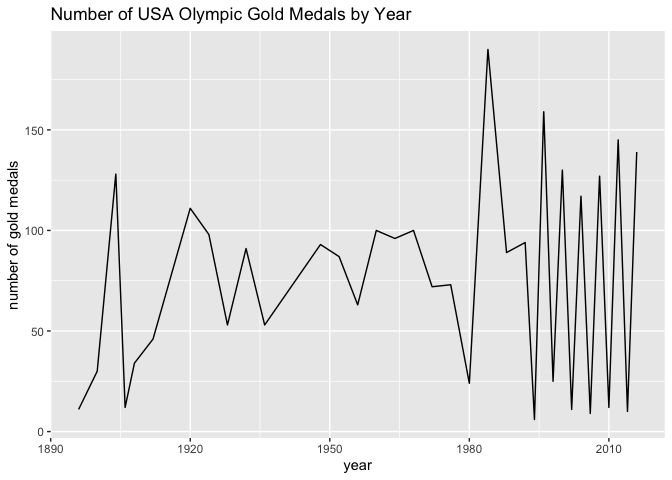
\includegraphics{HW3_files/figure-latex/unnamed-chunk-15-1.pdf}

The following genres of shows seem to last especially long: drama,
romance and crime, drama, mystery. Ratings do seem to change across
seasons.

\begin{Shaded}
\begin{Highlighting}[]
\NormalTok{tv\_long }\SpecialCharTok{\%\textgreater{}\%} 
  \FunctionTok{filter}\NormalTok{(genres}\SpecialCharTok{==}\StringTok{"Drama,Family,Fantasy"}\NormalTok{) }\SpecialCharTok{\%\textgreater{}\%} 
\NormalTok{  dplyr}\SpecialCharTok{::}\FunctionTok{select}\NormalTok{(title)}
\end{Highlighting}
\end{Shaded}

\begin{verbatim}
## # A tibble: 7 x 1
##   title                      
##   <chr>                      
## 1 Are You Afraid of the Dark?
## 2 Are You Afraid of the Dark?
## 3 Are You Afraid of the Dark?
## 4 Are You Afraid of the Dark?
## 5 Are You Afraid of the Dark?
## 6 Are You Afraid of the Dark?
## 7 Are You Afraid of the Dark?
\end{verbatim}

I assumed that the show that plummeted would be GOT, but it is actually
``Are You Afraid of the Dark?''.

\hypertarget{question-3-1}{%
\subsection{Question 3}\label{question-3-1}}

\begin{Shaded}
\begin{Highlighting}[]
\NormalTok{tv\_best }\OtherTok{\textless{}{-}}\NormalTok{ tv\_ratings }\SpecialCharTok{\%\textgreater{}\%} 
  \FunctionTok{filter}\NormalTok{(av\_rating}\SpecialCharTok{\textgreater{}=}\DecValTok{9}\NormalTok{)}
\end{Highlighting}
\end{Shaded}

\begin{Shaded}
\begin{Highlighting}[]
\NormalTok{tv\_best }\SpecialCharTok{\%\textgreater{}\%} 
  \FunctionTok{ggplot}\NormalTok{(}\FunctionTok{aes}\NormalTok{(}\AttributeTok{x=}\NormalTok{genres)) }\SpecialCharTok{+}
  \FunctionTok{geom\_bar}\NormalTok{() }\SpecialCharTok{+} \FunctionTok{theme\_minimal}\NormalTok{()}
\end{Highlighting}
\end{Shaded}

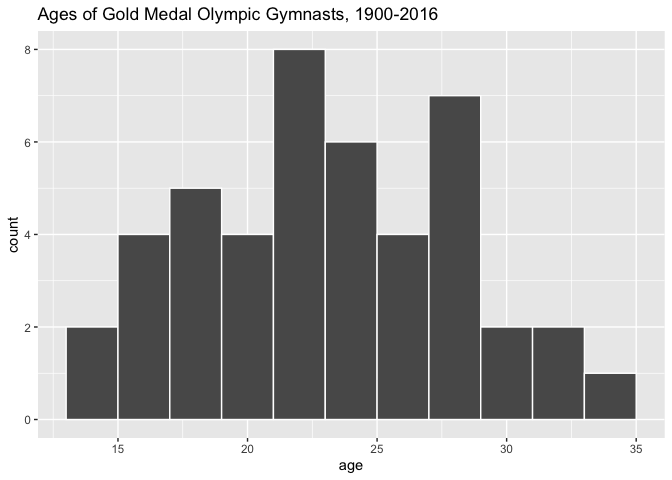
\includegraphics{HW3_files/figure-latex/unnamed-chunk-18-1.pdf}

First try, impossible to read the x-axis.

\begin{Shaded}
\begin{Highlighting}[]
\NormalTok{tv\_best }\SpecialCharTok{\%\textgreater{}\%} 
  \FunctionTok{ggplot}\NormalTok{(}\FunctionTok{aes}\NormalTok{(}\AttributeTok{x=}\NormalTok{genres)) }\SpecialCharTok{+}
  \FunctionTok{geom\_bar}\NormalTok{() }\SpecialCharTok{+}
  \FunctionTok{coord\_flip}\NormalTok{() }\SpecialCharTok{+} 
  \FunctionTok{theme\_minimal}\NormalTok{()}
\end{Highlighting}
\end{Shaded}

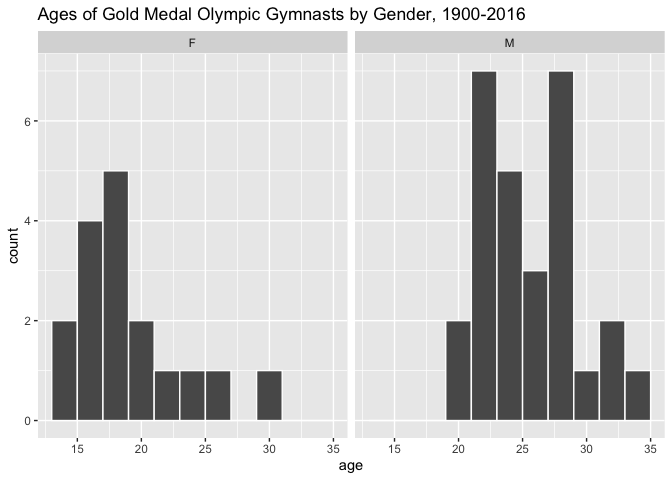
\includegraphics{HW3_files/figure-latex/unnamed-chunk-19-1.pdf}

\begin{Shaded}
\begin{Highlighting}[]
  \FunctionTok{labs}\NormalTok{(}\AttributeTok{title=}\StringTok{"Number of Show Seasons with an Avereage Rating of 9/10 or Greater by Genre"}\NormalTok{)}
\end{Highlighting}
\end{Shaded}

\begin{verbatim}
## $title
## [1] "Number of Show Seasons with an Avereage Rating of 9/10 or Greater by Genre"
## 
## attr(,"class")
## [1] "labels"
\end{verbatim}

Wow, much better. \texttt{coord\_flip} flips the coordinates so that the
original x-axis is shown on the y-axis and vice versa. Drama is the
genre with the most top-rated shows.

\hypertarget{question-4-1}{%
\subsection{Question 4}\label{question-4-1}}

\begin{Shaded}
\begin{Highlighting}[]
\NormalTok{comedies\_dramas }\OtherTok{\textless{}{-}}\NormalTok{ tv\_ratings }\SpecialCharTok{\%\textgreater{}\%} 
  \FunctionTok{mutate}\NormalTok{(}\AttributeTok{is\_comedy =} \FunctionTok{if\_else}\NormalTok{(}\FunctionTok{str\_detect}\NormalTok{(genres, }\StringTok{"Comedy"}\NormalTok{), }
                             \DecValTok{1}\NormalTok{, }
                             \DecValTok{0}\NormalTok{)) }\SpecialCharTok{\%\textgreater{}\%} \CommentTok{\# If it contains the word comedy then 1, else 0}
  \FunctionTok{filter}\NormalTok{(is\_comedy }\SpecialCharTok{==} \DecValTok{1} \SpecialCharTok{|}\NormalTok{ genres }\SpecialCharTok{==} \StringTok{"Drama"}\NormalTok{) }\SpecialCharTok{\%\textgreater{}\%} \CommentTok{\# Keep comedies and dramas}
  \FunctionTok{mutate}\NormalTok{(}\AttributeTok{genres =} \FunctionTok{if\_else}\NormalTok{(genres }\SpecialCharTok{==} \StringTok{"Drama"}\NormalTok{, }\CommentTok{\# Make it so that we only have those two genres}
                          \StringTok{"Drama"}\NormalTok{, }
                          \StringTok{"Comedy"}\NormalTok{))}

\FunctionTok{glimpse}\NormalTok{(comedies\_dramas)}
\end{Highlighting}
\end{Shaded}

\begin{verbatim}
## Rows: 684
## Columns: 8
## $ titleId      <chr> "tt0312081", "tt0312081", "tt0312081", "tt1225901", "tt12~
## $ seasonNumber <dbl> 1, 2, 3, 1, 2, 3, 4, 5, 1, 2, 1, 25, 1, 1, 2, 3, 4, 5, 1,~
## $ title        <chr> "8 Simple Rules", "8 Simple Rules", "8 Simple Rules", "90~
## $ date         <date> 2002-09-17, 2003-11-04, 2004-11-12, 2009-01-03, 2009-11-~
## $ av_rating    <dbl> 7.5000, 8.6000, 8.4043, 7.1735, 7.4686, 7.6858, 6.8344, 7~
## $ share        <dbl> 0.03, 0.10, 0.06, 0.40, 0.14, 0.10, 0.04, 0.01, 0.48, 0.4~
## $ genres       <chr> "Comedy", "Comedy", "Comedy", "Comedy", "Comedy", "Comedy~
## $ is_comedy    <dbl> 1, 1, 1, 1, 1, 1, 1, 1, 1, 1, 0, 1, 1, 1, 1, 1, 1, 1, 1, ~
\end{verbatim}

\begin{Shaded}
\begin{Highlighting}[]
\NormalTok{comedies\_dramas }\SpecialCharTok{\%\textgreater{}\%} 
  \FunctionTok{ggplot}\NormalTok{(}\FunctionTok{aes}\NormalTok{(}\AttributeTok{x=}\NormalTok{av\_rating,}
             \AttributeTok{fill=}\NormalTok{genres,}
             \AttributeTok{color=}\NormalTok{genres)) }\SpecialCharTok{+}
  \FunctionTok{geom\_density}\NormalTok{(}\AttributeTok{alpha=}\NormalTok{.}\DecValTok{3}\NormalTok{) }\SpecialCharTok{+}
  \FunctionTok{labs}\NormalTok{(}\AttributeTok{x=}\StringTok{"Average Rating"}\NormalTok{)}
\end{Highlighting}
\end{Shaded}

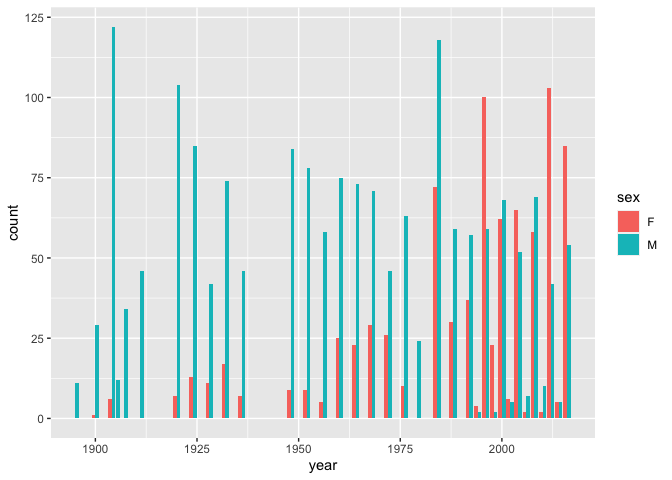
\includegraphics{HW3_files/figure-latex/unnamed-chunk-21-1.pdf}

No, sorry Nico, dramas have a slightly higher peak (most common rating),
and also have more extremely highly rated tv seasons than do comedies.

\hypertarget{question-5-1}{%
\subsection{Question 5}\label{question-5-1}}

\begin{Shaded}
\begin{Highlighting}[]
\NormalTok{comedies\_dramas }\SpecialCharTok{\%\textgreater{}\%} 
  \FunctionTok{ggplot}\NormalTok{(}\FunctionTok{aes}\NormalTok{(}\AttributeTok{x=}\NormalTok{av\_rating,}
             \AttributeTok{fill=}\NormalTok{genres,}
             \AttributeTok{color=}\NormalTok{genres)) }\SpecialCharTok{+}
  \FunctionTok{geom\_histogram}\NormalTok{(}\AttributeTok{alpha=}\NormalTok{.}\DecValTok{3}\NormalTok{) }\SpecialCharTok{+}
  \FunctionTok{labs}\NormalTok{(}\AttributeTok{x=}\StringTok{"Average Rating"}\NormalTok{)}
\end{Highlighting}
\end{Shaded}

\begin{verbatim}
## `stat_bin()` using `bins = 30`. Pick better value with `binwidth`.
\end{verbatim}

\includegraphics{HW3_files/figure-latex/unnamed-chunk-22-1.pdf}

The histogram is helpful because it shows raw counts and makes it clear
that we have many more comedies in our dataset than dramas. However, it
is difficult to compare the relative frequencies of different ratings.

\begin{Shaded}
\begin{Highlighting}[]
\NormalTok{comedies\_dramas }\SpecialCharTok{\%\textgreater{}\%} 
  \FunctionTok{ggplot}\NormalTok{(}\FunctionTok{aes}\NormalTok{(}\AttributeTok{x=}\NormalTok{av\_rating,}
             \AttributeTok{fill=}\NormalTok{genres,}
             \AttributeTok{color=}\NormalTok{genres)) }\SpecialCharTok{+}
  \FunctionTok{geom\_freqpoly}\NormalTok{(}\AttributeTok{alpha=}\NormalTok{.}\DecValTok{7}\NormalTok{) }\SpecialCharTok{+}
  \FunctionTok{labs}\NormalTok{(}\AttributeTok{x=}\StringTok{"Average Rating"}\NormalTok{)}
\end{Highlighting}
\end{Shaded}

\begin{verbatim}
## `stat_bin()` using `bins = 30`. Pick better value with `binwidth`.
\end{verbatim}

\includegraphics{HW3_files/figure-latex/unnamed-chunk-23-1.pdf}

This plot seems to show the same information as the histogram except
using lines in place of bars. I think that for our purposes, the density
plot is most informative because it accounts for the differences in the
number of observations for each genre.

\hypertarget{question-6-1}{%
\subsection{Question 6}\label{question-6-1}}

\begin{Shaded}
\begin{Highlighting}[]
\NormalTok{comedies\_dramas }\SpecialCharTok{\%\textgreater{}\%} 
  \FunctionTok{ggplot}\NormalTok{(}\FunctionTok{aes}\NormalTok{(}\AttributeTok{x=}\NormalTok{av\_rating, }\AttributeTok{y=}\NormalTok{share)) }\SpecialCharTok{+}
  \FunctionTok{geom\_bin\_2d}\NormalTok{() }\SpecialCharTok{+} 
  \FunctionTok{labs}\NormalTok{(}\AttributeTok{x=}\StringTok{"Average Rating"}\NormalTok{)}
\end{Highlighting}
\end{Shaded}

\includegraphics{HW3_files/figure-latex/unnamed-chunk-24-1.pdf}

This gives you information about the relationship between two different
variables and about the distribution of tv shows along these dimensions.
It also addresses issues related to overplotting in a scatterplot as the
fill gives information about the count of shows within each 2d bin. I'm
curious about the show with such a viewer share.

\begin{Shaded}
\begin{Highlighting}[]
\NormalTok{comedies\_dramas }\SpecialCharTok{\%\textgreater{}\%} 
  \FunctionTok{ggplot}\NormalTok{(}\FunctionTok{aes}\NormalTok{(}\AttributeTok{x=}\NormalTok{av\_rating, }\AttributeTok{y=}\NormalTok{share, }\AttributeTok{fill=}\NormalTok{genres)) }\SpecialCharTok{+}
  \FunctionTok{geom\_bin\_2d}\NormalTok{() }\SpecialCharTok{+}
  \FunctionTok{labs}\NormalTok{(}\AttributeTok{x=}\StringTok{"Average Rating"}\NormalTok{)}
\end{Highlighting}
\end{Shaded}

\includegraphics{HW3_files/figure-latex/unnamed-chunk-25-1.pdf}

Comedy shows with lower ratings tend to have higher viewership shares
than do dramas with higher ratings, which is interesting (besides the
one outlier).

\begin{Shaded}
\begin{Highlighting}[]
\NormalTok{ mystery\_show }\OtherTok{\textless{}{-}}\NormalTok{ comedies\_dramas }\SpecialCharTok{\%\textgreater{}\%} 
  \FunctionTok{filter}\NormalTok{(share}\SpecialCharTok{\textgreater{}}\DecValTok{20}\NormalTok{) }
\end{Highlighting}
\end{Shaded}

The show is ``Dekalog.'' Never heard of it\ldots{}

\hypertarget{just-for-fun}{%
\subsection{Just for fun}\label{just-for-fun}}

\begin{Shaded}
\begin{Highlighting}[]
\NormalTok{got }\OtherTok{\textless{}{-}}\NormalTok{ tv\_ratings }\SpecialCharTok{\%\textgreater{}\%} 
  \FunctionTok{filter}\NormalTok{(title}\SpecialCharTok{==}\StringTok{"Game of Thrones"}\NormalTok{)}

\NormalTok{got }\SpecialCharTok{\%\textgreater{}\%} 
  \FunctionTok{ggplot}\NormalTok{(}\FunctionTok{aes}\NormalTok{(}\AttributeTok{x=}\NormalTok{seasonNumber,}
             \AttributeTok{y=}\NormalTok{av\_rating)) }\SpecialCharTok{+}
  \FunctionTok{geom\_line}\NormalTok{(}\AttributeTok{color=}\StringTok{"red"}\NormalTok{) }\SpecialCharTok{+}
  \FunctionTok{labs}\NormalTok{(}\AttributeTok{x=}\StringTok{"Season"}\NormalTok{,}
       \AttributeTok{y=}\StringTok{"Average Rating"}\NormalTok{,}
       \AttributeTok{title=}\StringTok{"Game of Thrones Average Rating by Season"}\NormalTok{) }\SpecialCharTok{+}\FunctionTok{ylim}\NormalTok{(}\DecValTok{8}\NormalTok{, }\DecValTok{10}\NormalTok{)}
\end{Highlighting}
\end{Shaded}

\includegraphics{HW3_files/figure-latex/unnamed-chunk-27-1.pdf}

\hypertarget{dv-5}{%
\section{DV 5}\label{dv-5}}

\begin{Shaded}
\begin{Highlighting}[]
\FunctionTok{library}\NormalTok{(tidyverse)}
\CommentTok{\# Read in the data }
\NormalTok{wncaa }\OtherTok{\textless{}{-}} \FunctionTok{read\_csv}\NormalTok{(}\StringTok{"Data/wncaa.csv"}\NormalTok{)}
\end{Highlighting}
\end{Shaded}

\begin{verbatim}
## Rows: 2092 Columns: 19
## -- Column specification --------------------------------------------------------
## Delimiter: ","
## chr  (6): school, conference, conf_place, how_qual, x1st_game_at_home, tourn...
## dbl (13): year, seed, conf_w, conf_l, conf_percent, reg_w, reg_l, reg_percen...
## 
## i Use `spec()` to retrieve the full column specification for this data.
## i Specify the column types or set `show_col_types = FALSE` to quiet this message.
\end{verbatim}

\begin{Shaded}
\begin{Highlighting}[]
\CommentTok{\# Glimpse the data }
\FunctionTok{glimpse}\NormalTok{(wncaa)}
\end{Highlighting}
\end{Shaded}

\begin{verbatim}
## Rows: 2,092
## Columns: 19
## $ year              <dbl> 1982, 1982, 1982, 1982, 1982, 1982, 1982, 1982, 1982~
## $ school            <chr> "Arizona St.", "Auburn", "Cheyney", "Clemson", "Drak~
## $ seed              <dbl> 4, 7, 2, 5, 4, 6, 5, 8, 7, 7, 4, 8, 2, 1, 1, 2, 3, 6~
## $ conference        <chr> "Western Collegiate", "Southeastern", "Independent",~
## $ conf_w            <dbl> NA, NA, NA, 6, NA, NA, NA, NA, NA, NA, NA, NA, NA, N~
## $ conf_l            <dbl> NA, NA, NA, 3, NA, NA, NA, NA, NA, NA, NA, NA, NA, N~
## $ conf_percent      <dbl> NA, NA, NA, 66.7, NA, NA, NA, NA, NA, NA, NA, NA, NA~
## $ conf_place        <chr> "-", "-", "-", "4th", "-", "-", "-", "-", "-", "-", ~
## $ reg_w             <dbl> 23, 24, 24, 20, 26, 19, 21, 14, 21, 28, 24, 17, 22, ~
## $ reg_l             <dbl> 6, 4, 2, 11, 6, 7, 8, 10, 8, 7, 5, 13, 7, 5, 1, 6, 4~
## $ reg_percent       <dbl> 79.3, 85.7, 92.3, 64.5, 81.3, 73.1, 72.4, 58.3, 72.4~
## $ how_qual          <chr> "at-large", "at-large", "at-large", "at-large", "aut~
## $ x1st_game_at_home <chr> "Y", "N", "Y", "N", "Y", "N", "N", "N", "N", "N", "Y~
## $ tourney_w         <dbl> 1, 0, 4, 0, 2, 0, 0, 0, 0, 0, 2, 0, 2, 1, 5, 3, 1, 1~
## $ tourney_l         <dbl> 1, 1, 1, 1, 1, 1, 1, 1, 1, 1, 1, 1, 1, 1, 0, 1, 1, 1~
## $ tourney_finish    <chr> "RSF", "1st", "N2nd", "1st", "RF", "1st", "1st", "1s~
## $ full_w            <dbl> 24, 24, 28, 20, 28, 19, 21, 14, 21, 28, 26, 17, 24, ~
## $ full_l            <dbl> 7, 5, 3, 12, 7, 8, 9, 11, 9, 8, 6, 14, 8, 6, 1, 7, 5~
## $ full_percent      <dbl> 77.4, 82.8, 90.3, 62.5, 80.0, 70.4, 70.0, 56.0, 70.0~
\end{verbatim}

\hypertarget{question-1-2}{%
\subsection{Question 1}\label{question-1-2}}

\begin{Shaded}
\begin{Highlighting}[]
\NormalTok{tourney\_wins }\OtherTok{\textless{}{-}}\NormalTok{ wncaa }\SpecialCharTok{\%\textgreater{}\%} 
  \FunctionTok{filter}\NormalTok{(tourney\_finish}\SpecialCharTok{==}\StringTok{"Champ"}\NormalTok{) }\SpecialCharTok{\%\textgreater{}\%} 
  \FunctionTok{group\_by}\NormalTok{(school) }\SpecialCharTok{\%\textgreater{}\%} 
  \FunctionTok{summarize}\NormalTok{(}\AttributeTok{N=}\FunctionTok{n}\NormalTok{()) }\SpecialCharTok{\%\textgreater{}\%} 
  \FunctionTok{mutate}\NormalTok{(}\AttributeTok{freq=}\NormalTok{N}\SpecialCharTok{/} \FunctionTok{sum}\NormalTok{(N),}
         \AttributeTok{pct=} \FunctionTok{round}\NormalTok{((freq}\SpecialCharTok{*}\DecValTok{100}\NormalTok{), }\DecValTok{0}\NormalTok{)) }
\end{Highlighting}
\end{Shaded}

\begin{Shaded}
\begin{Highlighting}[]
\NormalTok{tourney\_wins }\SpecialCharTok{\%\textgreater{}\%} 
  \FunctionTok{ggplot}\NormalTok{(}\FunctionTok{aes}\NormalTok{(}\AttributeTok{x=}\FunctionTok{reorder}\NormalTok{(school, pct), }\AttributeTok{y=}\NormalTok{pct)) }\SpecialCharTok{+}
  \FunctionTok{geom\_col}\NormalTok{(}\AttributeTok{position=}\StringTok{"dodge"}\NormalTok{) }\SpecialCharTok{+}
  \FunctionTok{coord\_flip}\NormalTok{() }\SpecialCharTok{+} 
  \FunctionTok{labs}\NormalTok{(}\AttributeTok{x=}\ConstantTok{NULL}\NormalTok{, }\AttributeTok{y=}\StringTok{"Percent"}\NormalTok{,}
       \AttributeTok{title=}\StringTok{"Share of WNCAA Tournament Wins by School"}\NormalTok{) }\SpecialCharTok{+}
  \FunctionTok{theme\_minimal}\NormalTok{()}
\end{Highlighting}
\end{Shaded}

\includegraphics{HW3_files/figure-latex/unnamed-chunk-30-1.pdf}
Together, UConn and Tennessee have won the majority of WNCAA
tournaments. The rest of these teams have won a significantly lower
percentage of tournaments.

\hypertarget{question-2-1}{%
\subsection{Question 2}\label{question-2-1}}

\begin{Shaded}
\begin{Highlighting}[]
\NormalTok{champ\_names }\OtherTok{\textless{}{-}} \FunctionTok{unique}\NormalTok{(tourney\_wins}\SpecialCharTok{$}\NormalTok{school)}

\NormalTok{winners }\OtherTok{\textless{}{-}}\NormalTok{ wncaa }\SpecialCharTok{\%\textgreater{}\%} 
  \FunctionTok{filter}\NormalTok{(school }\SpecialCharTok{\%in\%}\NormalTok{ champ\_names)}
\end{Highlighting}
\end{Shaded}

\begin{Shaded}
\begin{Highlighting}[]
\NormalTok{winners }\SpecialCharTok{\%\textgreater{}\%} \FunctionTok{ggplot}\NormalTok{(}\FunctionTok{aes}\NormalTok{(}\AttributeTok{x=}\FunctionTok{reorder}\NormalTok{(school, seed, }\AttributeTok{na.rm=}\ConstantTok{TRUE}\NormalTok{),}
                       \AttributeTok{y=}\NormalTok{seed)) }\SpecialCharTok{+}
  \FunctionTok{geom\_boxplot}\NormalTok{() }\SpecialCharTok{+}
  \FunctionTok{coord\_flip}\NormalTok{() }\SpecialCharTok{+} 
  \FunctionTok{labs}\NormalTok{(}\AttributeTok{x=}\ConstantTok{NULL}\NormalTok{) }\SpecialCharTok{+}
  \FunctionTok{theme\_minimal}\NormalTok{()}
\end{Highlighting}
\end{Shaded}

\includegraphics{HW3_files/figure-latex/unnamed-chunk-32-1.pdf}

Honestly, don't know what seeds are. Based on my brief read on the
subject we would expect UConn and Tennessee to have low seeds.
Interesting that Notre Dame has the second highest mean and median given
they are in the second tier of schools based on the graph from Q1.

\begin{Shaded}
\begin{Highlighting}[]
\NormalTok{winners }\SpecialCharTok{\%\textgreater{}\%} \FunctionTok{ggplot}\NormalTok{(}\FunctionTok{aes}\NormalTok{(}\AttributeTok{x=}\FunctionTok{reorder}\NormalTok{(school, seed, }\AttributeTok{na.rm=}\ConstantTok{TRUE}\NormalTok{),}
                       \AttributeTok{y=}\NormalTok{seed)) }\SpecialCharTok{+}
  \FunctionTok{geom\_violin}\NormalTok{() }\SpecialCharTok{+}
  \FunctionTok{coord\_flip}\NormalTok{() }\SpecialCharTok{+} 
  \FunctionTok{labs}\NormalTok{(}\AttributeTok{x=}\ConstantTok{NULL}\NormalTok{) }\SpecialCharTok{+}
  \FunctionTok{theme\_minimal}\NormalTok{()}
\end{Highlighting}
\end{Shaded}

\includegraphics{HW3_files/figure-latex/unnamed-chunk-33-1.pdf}

I personally find the boxplot more informative and digestible but I
appreciate that the violin plot also shows the full distribution of
data.

\hypertarget{question-3-2}{%
\subsection{Question 3}\label{question-3-2}}

\begin{Shaded}
\begin{Highlighting}[]
\NormalTok{winners }\SpecialCharTok{\%\textgreater{}\%} \FunctionTok{ggplot}\NormalTok{(}\FunctionTok{aes}\NormalTok{(}\AttributeTok{x=}\FunctionTok{reorder}\NormalTok{(school, seed, }\AttributeTok{na.rm=}\ConstantTok{TRUE}\NormalTok{),}
                       \AttributeTok{y=}\NormalTok{seed)) }\SpecialCharTok{+}
  \FunctionTok{geom\_point}\NormalTok{() }\SpecialCharTok{+}
  \FunctionTok{coord\_flip}\NormalTok{() }\SpecialCharTok{+} 
  \FunctionTok{labs}\NormalTok{(}\AttributeTok{x=}\ConstantTok{NULL}\NormalTok{) }\SpecialCharTok{+}
  \FunctionTok{theme\_minimal}\NormalTok{()}
\end{Highlighting}
\end{Shaded}

\includegraphics{HW3_files/figure-latex/unnamed-chunk-34-1.pdf}

This is not helpful because seed only takes interger values and it's
impossible to tell how many observations occurred at each seed value;
this only shows if there was at least one seed set at a given value.

\hypertarget{question-4-2}{%
\subsection{Question 4}\label{question-4-2}}

\begin{Shaded}
\begin{Highlighting}[]
\NormalTok{winners\_sts }\OtherTok{\textless{}{-}}\NormalTok{ winners }\SpecialCharTok{\%\textgreater{}\%} \FunctionTok{group\_by}\NormalTok{(school) }\SpecialCharTok{\%\textgreater{}\%} 
  \FunctionTok{summarize\_if}\NormalTok{(is.numeric, }\FunctionTok{funs}\NormalTok{(mean, sd), }\AttributeTok{na.rm =} \ConstantTok{TRUE}\NormalTok{) }\SpecialCharTok{\%\textgreater{}\%}
  \FunctionTok{ungroup}\NormalTok{()}
\end{Highlighting}
\end{Shaded}

\begin{verbatim}
## Warning: `funs()` was deprecated in dplyr 0.8.0.
## Please use a list of either functions or lambdas: 
## 
##   # Simple named list: 
##   list(mean = mean, median = median)
## 
##   # Auto named with `tibble::lst()`: 
##   tibble::lst(mean, median)
## 
##   # Using lambdas
##   list(~ mean(., trim = .2), ~ median(., na.rm = TRUE))
## This warning is displayed once every 8 hours.
## Call `lifecycle::last_lifecycle_warnings()` to see where this warning was generated.
\end{verbatim}

\begin{Shaded}
\begin{Highlighting}[]
\NormalTok{winners\_sts }\SpecialCharTok{\%\textgreater{}\%} 
  \FunctionTok{ggplot}\NormalTok{(}\FunctionTok{aes}\NormalTok{(}\AttributeTok{x=}\FunctionTok{reorder}\NormalTok{(school, reg\_percent\_mean),}
             \AttributeTok{y=}\NormalTok{reg\_percent\_mean)) }\SpecialCharTok{+}
  \FunctionTok{geom\_point}\NormalTok{(}\AttributeTok{size=}\DecValTok{3}\NormalTok{) }\SpecialCharTok{+}
  \FunctionTok{coord\_flip}\NormalTok{() }\SpecialCharTok{+}
  \FunctionTok{theme\_minimal}\NormalTok{() }\SpecialCharTok{+}
  \FunctionTok{labs}\NormalTok{(}\AttributeTok{x=}\ConstantTok{NULL}\NormalTok{, }
       \AttributeTok{y=}\StringTok{"average win percentage"}\NormalTok{)}
\end{Highlighting}
\end{Shaded}

\includegraphics{HW3_files/figure-latex/unnamed-chunk-35-1.pdf}

Interesting that while UConn remains in the top two in terms of average
win percentage, Tennessee is not in the top two based on this statistic.

\begin{Shaded}
\begin{Highlighting}[]
\NormalTok{winners\_sts }\SpecialCharTok{\%\textgreater{}\%} 
  \FunctionTok{ggplot}\NormalTok{(}\FunctionTok{aes}\NormalTok{(}\AttributeTok{x=}\FunctionTok{reorder}\NormalTok{(school, reg\_percent\_mean),}
             \AttributeTok{y=}\NormalTok{reg\_percent\_mean)) }\SpecialCharTok{+}
  \FunctionTok{geom\_pointrange}\NormalTok{(}\FunctionTok{aes}\NormalTok{(}\AttributeTok{ymin=}\NormalTok{reg\_percent\_mean}\SpecialCharTok{{-}}\NormalTok{reg\_percent\_sd,}
                      \AttributeTok{ymax=}\NormalTok{reg\_percent\_mean}\SpecialCharTok{+}\NormalTok{reg\_percent\_sd)) }\SpecialCharTok{+}
  \FunctionTok{coord\_flip}\NormalTok{() }\SpecialCharTok{+}
  \FunctionTok{theme\_minimal}\NormalTok{() }\SpecialCharTok{+}
  \FunctionTok{labs}\NormalTok{(}\AttributeTok{x=}\ConstantTok{NULL}\NormalTok{, }
       \AttributeTok{y=}\StringTok{"average win percentage and standard deviation"}\NormalTok{)}
\end{Highlighting}
\end{Shaded}

\includegraphics{HW3_files/figure-latex/unnamed-chunk-36-1.pdf}

Texas A\&M has the most narrow interval.

\begin{Shaded}
\begin{Highlighting}[]
\NormalTok{p }\OtherTok{\textless{}{-}}\NormalTok{ winners\_sts }\SpecialCharTok{\%\textgreater{}\%} 
  \FunctionTok{ggplot}\NormalTok{(}\FunctionTok{aes}\NormalTok{(}\AttributeTok{x=}\FunctionTok{reorder}\NormalTok{(school, reg\_percent\_mean),}
             \AttributeTok{y=}\NormalTok{reg\_percent\_mean)) }\SpecialCharTok{+}
  \FunctionTok{geom\_point}\NormalTok{(}\AttributeTok{size=}\DecValTok{3}\NormalTok{)}

\NormalTok{p }\SpecialCharTok{+} \FunctionTok{geom\_linerange}\NormalTok{(}\FunctionTok{aes}\NormalTok{(}\AttributeTok{ymin=}\NormalTok{reg\_percent\_mean}\SpecialCharTok{{-}}\NormalTok{reg\_percent\_sd,}
                      \AttributeTok{ymax=}\NormalTok{reg\_percent\_mean}\SpecialCharTok{+}\NormalTok{reg\_percent\_sd)) }\SpecialCharTok{+}
  \FunctionTok{coord\_flip}\NormalTok{() }\SpecialCharTok{+}
  \FunctionTok{theme\_minimal}\NormalTok{() }\SpecialCharTok{+}
  \FunctionTok{labs}\NormalTok{(}\AttributeTok{x=}\ConstantTok{NULL}\NormalTok{, }
       \AttributeTok{y=}\StringTok{"average win percentage and standard deviation"}\NormalTok{)}
\end{Highlighting}
\end{Shaded}

\includegraphics{HW3_files/figure-latex/unnamed-chunk-37-1.pdf}

\hypertarget{question-5-2}{%
\subsection{Question 5}\label{question-5-2}}

\begin{Shaded}
\begin{Highlighting}[]
\NormalTok{winners }\SpecialCharTok{\%\textgreater{}\%} \FunctionTok{ggplot}\NormalTok{(}\FunctionTok{aes}\NormalTok{(}\AttributeTok{x=}\NormalTok{reg\_percent,}
                   \AttributeTok{y=}\NormalTok{full\_percent)) }\SpecialCharTok{+}
  \FunctionTok{geom\_point}\NormalTok{(}\AttributeTok{alpha=}\NormalTok{.}\DecValTok{3}\NormalTok{) }\SpecialCharTok{+}
  \FunctionTok{geom\_abline}\NormalTok{() }\SpecialCharTok{+}
  \FunctionTok{theme\_minimal}\NormalTok{() }\SpecialCharTok{+}
  \FunctionTok{xlim}\NormalTok{(}\DecValTok{0}\NormalTok{,}\DecValTok{100}\NormalTok{) }\SpecialCharTok{+}
  \FunctionTok{ylim}\NormalTok{(}\DecValTok{0}\NormalTok{,}\DecValTok{100}\NormalTok{) }\SpecialCharTok{+}
  \FunctionTok{labs}\NormalTok{(}\AttributeTok{x=}\StringTok{"WNCAA Regular Season \% Wins"}\NormalTok{, }
       \AttributeTok{y=}\StringTok{"WNCAA Full Season \% Wins"}\NormalTok{)}
\end{Highlighting}
\end{Shaded}

\includegraphics{HW3_files/figure-latex/unnamed-chunk-38-1.pdf}

Most dots are below the line as expected. Dots above the line occur
mostly at the upper bounds of reg\_percent, so it seems that teams that
overperform at tournaments also tend to do quite well during the regular
season.

\hypertarget{question-6-2}{%
\subsection{Question 6}\label{question-6-2}}

\begin{Shaded}
\begin{Highlighting}[]
\NormalTok{winners }\OtherTok{\textless{}{-}}\NormalTok{ winners }\SpecialCharTok{\%\textgreater{}\%} 
  \FunctionTok{mutate}\NormalTok{(}\AttributeTok{is\_champ =} \FunctionTok{if\_else}\NormalTok{(tourney\_finish }\SpecialCharTok{==} \StringTok{"Champ"}\NormalTok{, }\DecValTok{1}\NormalTok{, }\DecValTok{0}\NormalTok{), }
         \AttributeTok{is\_champ =} \FunctionTok{as.factor}\NormalTok{(is\_champ))}
\NormalTok{winners }\SpecialCharTok{\%\textgreater{}\%} \FunctionTok{ggplot}\NormalTok{(}\FunctionTok{aes}\NormalTok{(}\AttributeTok{x=}\NormalTok{reg\_percent,}
                   \AttributeTok{y=}\NormalTok{full\_percent,}
                   \AttributeTok{color=}\NormalTok{is\_champ)) }\SpecialCharTok{+}
  \FunctionTok{geom\_point}\NormalTok{(}\AttributeTok{alpha=}\NormalTok{.}\DecValTok{3}\NormalTok{) }\SpecialCharTok{+}
  \FunctionTok{geom\_abline}\NormalTok{() }\SpecialCharTok{+}
  \FunctionTok{theme\_minimal}\NormalTok{() }\SpecialCharTok{+}
  \FunctionTok{xlim}\NormalTok{(}\DecValTok{0}\NormalTok{,}\DecValTok{100}\NormalTok{) }\SpecialCharTok{+}
  \FunctionTok{ylim}\NormalTok{(}\DecValTok{0}\NormalTok{,}\DecValTok{100}\NormalTok{) }\SpecialCharTok{+}
  \FunctionTok{labs}\NormalTok{(}\AttributeTok{x=}\StringTok{"WNCAA Regular Season \% Wins"}\NormalTok{, }
       \AttributeTok{y=}\StringTok{"WNCAA Full Season \% Wins"}\NormalTok{)}
\end{Highlighting}
\end{Shaded}

\includegraphics{HW3_files/figure-latex/unnamed-chunk-39-1.pdf}

Wow, almost all of the dots above the line represent teams that were
champions in their tournament that year. This makes sense because they
won the tournament which is why their full season percentage of wins is
higher than the regular season percentage.

\begin{Shaded}
\begin{Highlighting}[]
\NormalTok{winners }\OtherTok{\textless{}{-}}\NormalTok{ winners }\SpecialCharTok{\%\textgreater{}\%} 
  \FunctionTok{mutate}\NormalTok{(}\AttributeTok{is\_champ =} \FunctionTok{if\_else}\NormalTok{(tourney\_finish }\SpecialCharTok{==} \StringTok{"Champ"}\NormalTok{, }\DecValTok{1}\NormalTok{, }\DecValTok{0}\NormalTok{))}
\NormalTok{winners }\SpecialCharTok{\%\textgreater{}\%} \FunctionTok{ggplot}\NormalTok{(}\FunctionTok{aes}\NormalTok{(}\AttributeTok{x=}\NormalTok{reg\_percent,}
                   \AttributeTok{y=}\NormalTok{full\_percent,}
                   \AttributeTok{color=}\NormalTok{is\_champ)) }\SpecialCharTok{+}
  \FunctionTok{geom\_point}\NormalTok{(}\AttributeTok{alpha=}\NormalTok{.}\DecValTok{3}\NormalTok{) }\SpecialCharTok{+}
  \FunctionTok{geom\_abline}\NormalTok{() }\SpecialCharTok{+}
  \FunctionTok{theme\_minimal}\NormalTok{() }\SpecialCharTok{+}
  \FunctionTok{xlim}\NormalTok{(}\DecValTok{0}\NormalTok{,}\DecValTok{100}\NormalTok{) }\SpecialCharTok{+}
  \FunctionTok{ylim}\NormalTok{(}\DecValTok{0}\NormalTok{,}\DecValTok{100}\NormalTok{) }\SpecialCharTok{+} 
  \FunctionTok{labs}\NormalTok{(}\AttributeTok{x=}\StringTok{"WNCAA Regular Season \% Wins"}\NormalTok{, }
       \AttributeTok{y=}\StringTok{"WNCAA Full Season \% Wins"}\NormalTok{)}
\end{Highlighting}
\end{Shaded}

\includegraphics{HW3_files/figure-latex/unnamed-chunk-40-1.pdf}

Without knowing that is\_champ is a factor variable, R assumes that it
is continuous and colors points with a continuous color scale. You can
still see the same patterns but the legend would be confusing for
someone else to see because it implies that is\_champ can take on values
other than 0 or 1, which is not the case.

\hypertarget{question-7-1}{%
\subsection{Question 7}\label{question-7-1}}

\begin{Shaded}
\begin{Highlighting}[]
\NormalTok{winners }\OtherTok{\textless{}{-}}\NormalTok{ winners }\SpecialCharTok{\%\textgreater{}\%} 
  \FunctionTok{mutate}\NormalTok{(}\AttributeTok{plot\_label =} \FunctionTok{paste}\NormalTok{(school, year, }\AttributeTok{sep =} \StringTok{"{-}"}\NormalTok{))}
\NormalTok{winners }\OtherTok{\textless{}{-}}\NormalTok{ winners }\SpecialCharTok{\%\textgreater{}\%} 
  \FunctionTok{mutate}\NormalTok{(}\AttributeTok{difference =}\NormalTok{ full\_percent }\SpecialCharTok{{-}}\NormalTok{ reg\_percent) }
\end{Highlighting}
\end{Shaded}

\begin{Shaded}
\begin{Highlighting}[]
\FunctionTok{library}\NormalTok{(ggrepel)}
\NormalTok{winners}\SpecialCharTok{$}\NormalTok{plot }\OtherTok{\textless{}{-}}\NormalTok{ winners}\SpecialCharTok{$}\NormalTok{reg\_percent}\SpecialCharTok{\textless{}}\DecValTok{50} \SpecialCharTok{|}\NormalTok{ (winners}\SpecialCharTok{$}\NormalTok{reg\_percent}\SpecialCharTok{\textless{}}\DecValTok{75} \SpecialCharTok{\&}\NormalTok{ winners}\SpecialCharTok{$}\NormalTok{is\_champ}\SpecialCharTok{==}\DecValTok{1}\NormalTok{)}
\NormalTok{p1 }\OtherTok{\textless{}{-}}\NormalTok{ winners }\SpecialCharTok{\%\textgreater{}\%} \FunctionTok{ggplot}\NormalTok{(}\FunctionTok{aes}\NormalTok{(}\AttributeTok{x=}\NormalTok{reg\_percent,}
                       \AttributeTok{y=}\NormalTok{full\_percent)) }
\NormalTok{p1 }\SpecialCharTok{+} \FunctionTok{geom\_point}\NormalTok{() }\SpecialCharTok{+}
  \FunctionTok{geom\_text\_repel}\NormalTok{(}\AttributeTok{data=}\FunctionTok{subset}\NormalTok{(winners, plot),}
                  \AttributeTok{mapping=}\FunctionTok{aes}\NormalTok{(}\AttributeTok{label=}\NormalTok{plot\_label), }\AttributeTok{nudge\_x=}\SpecialCharTok{{-}}\NormalTok{.}\DecValTok{2}\NormalTok{) }\SpecialCharTok{+}
  \FunctionTok{geom\_abline}\NormalTok{() }\SpecialCharTok{+}
  \FunctionTok{theme\_minimal}\NormalTok{() }\SpecialCharTok{+}
  \FunctionTok{labs}\NormalTok{(}\AttributeTok{x=}\StringTok{"WNCAA Regular Season \% Wins"}\NormalTok{, }
       \AttributeTok{y=}\StringTok{"WNCAA Full Season \% Wins"}\NormalTok{)}
\end{Highlighting}
\end{Shaded}

\includegraphics{HW3_files/figure-latex/unnamed-chunk-42-1.pdf}

I have labeled the points of interest, but just those two.

\begin{Shaded}
\begin{Highlighting}[]
\NormalTok{winners }\SpecialCharTok{\%\textgreater{}\%} \FunctionTok{filter}\NormalTok{(reg\_percent}\SpecialCharTok{==}\DecValTok{100} \SpecialCharTok{\&}\NormalTok{ full\_percent}\SpecialCharTok{==}\DecValTok{100}\NormalTok{) }\SpecialCharTok{\%\textgreater{}\%} 
\NormalTok{  dplyr}\SpecialCharTok{::}\FunctionTok{select}\NormalTok{ (plot\_label)}
\end{Highlighting}
\end{Shaded}

\begin{verbatim}
## # A tibble: 8 x 1
##   plot_label 
##   <chr>      
## 1 Texas-1986 
## 2 UConn-1995 
## 3 UConn-2002 
## 4 UConn-2009 
## 5 UConn-2010 
## 6 Baylor-2012
## 7 UConn-2014 
## 8 UConn-2016
\end{verbatim}

Most of the observations in which teams have won 100\% of regular and
fulls season games are UConn, which isn't surprising because previous
questions have shown that they are an extremely strong team. Texas is
the most surprising (and to a lesser extent Baylor) because they have a
much lower average win percentage and have won a much lower share of
tournaments than UConn.

\end{document}
